\documentclass{article}
\usepackage[hidelinks]{hyperref}
\usepackage[spanish,mexico]{babel}
\usepackage[raggedright]{titlesec}
\usepackage{listingsutf8}
\usepackage{color}
\usepackage[svgnames]{xcolor}
\usepackage[most]{tcolorbox}
\usepackage[tikz]{bclogo}
\usepackage{pst-blur}
\usepackage{graphicx}
\graphicspath{ {images/} }
\usepackage{fancyhdr}
\usepackage{hyphenat}
\usepackage[font=small,
            labelfont={bf,it},
            textfont=it]{caption}

\pagestyle{fancy}
\fancyhf{}
\rfoot{pág. \thepage}

\renewcommand\lstlistingname{Fig.}
\addto\captionsspanish{\renewcommand{\figurename}{Diagrama}}
\renewcommand{\headrulewidth}{0pt}

\newcommand{\code}[1]{\tcbox{\texttt{#1}}}
\newcommand{\codejs}[1]{\tcbox{\lstinline[style=ES6]{#1}}}
\newcommand{\operator}[2]{\item \textbf{#1} \codejs{#2}:}
\newcommand{\jsfile}[2]{\lstinputlisting[style=ES6, caption={#1}]{#2}}
\newcommand{\aparef}[2]{\href{#1}{#2 #1}}

\colorlet{lightgray}{gray!20}
\tcbset{on line, 
        boxsep=4pt, left=0pt,right=0pt,top=0pt,bottom=0pt,
        colframe=white,colback=lightgray,  
        highlight math style={enhanced}
}

\lstset{
     literate=%
         {á}{{\'a}}1
         {í}{{\'i}}1
         {é}{{\'e}}1
         {ý}{{\'y}}1
         {ú}{{\'u}}1
         {ó}{{\'o}}1
         {ě}{{\v{e}}}1
         {š}{{\v{s}}}1
         {č}{{\v{c}}}1
         {ř}{{\v{r}}}1
         {ž}{{\v{z}}}1
         {ď}{{\v{d}}}1
         {ť}{{\v{t}}}1
         {ň}{{\v{n}}}1                
         {ů}{{\r{u}}}1
         {Á}{{\'A}}1
         {Í}{{\'I}}1
         {É}{{\'E}}1
         {Ý}{{\'Y}}1
         {Ú}{{\'U}}1
         {Ó}{{\'O}}1
         {Ě}{{\v{E}}}1
         {Š}{{\v{S}}}1
         {Č}{{\v{C}}}1
         {Ř}{{\v{R}}}1
         {Ž}{{\v{Z}}}1
         {Ď}{{\v{D}}}1
         {Ť}{{\v{T}}}1
         {Ň}{{\v{N}}}1                
         {Ů}{{\r{U}}}1    
}
\lstset{framesep=10pt}
\lstset{xleftmargin=10pt,xrightmargin=10pt}

\lstalias[]{ES6}[ECMAScript2015]{JavaScript}
\lstdefinelanguage{JavaScript}{
  morekeywords=[1]{break, continue, delete, else, for, function, if, in,
    new, return, this, typeof, var, void, while, with},
  % Literals, primitive types, and reference types.
  morekeywords=[2]{false, null, true, boolean, undefined,
    Array, Boolean, Date, Math, Number, String, Object},
  % Built-ins.
  morekeywords=[3]{eval, parseInt, parseFloat, escape, unescape},
  sensitive,
  morecomment=[s]{/*}{*/},
  morecomment=[l]//,
  morecomment=[s]{/**}{*/}, % JavaDoc style comments
  morestring=[b]',
  morestring=[b]"
}[keywords, comments, strings]

\lstdefinelanguage[ECMAScript2015]{JavaScript}[]{JavaScript}{
  morekeywords=[1]{await, async, case, catch, class, const, default, do,
    enum, export, extends, finally, from, implements, import, instanceof,
    let, static, super, switch, throw, try},
  morestring=[b]` % Interpolation strings.
}

\definecolor{mediumgray}{rgb}{0.3, 0.4, 0.4}
\definecolor{mediumblue}{rgb}{0.0, 0.0, 0.8}
\definecolor{forestgreen}{rgb}{0.13, 0.55, 0.13}
\definecolor{darkviolet}{rgb}{0.58, 0.0, 0.83}
\definecolor{royalblue}{rgb}{0.25, 0.41, 0.88}
\definecolor{crimson}{rgb}{0.86, 0.8, 0.24}

\lstdefinestyle{JSES6Base}{
  backgroundcolor=\color{white},
  basicstyle=\ttfamily,
  breakatwhitespace=false,
  breaklines=false,
  captionpos=b,
  %abovecaptionskip=\medskipamount,
  columns=fullflexible,
  commentstyle=\color{mediumgray}\upshape,
  emph={},
  emphstyle=\color{crimson},
  extendedchars=true,  % requires inputenc
  fontadjust=true,
  frame=single,
  identifierstyle=\color{black},
  keepspaces=true,
  keywordstyle=\color{mediumblue},
  keywordstyle={[2]\color{darkviolet}},
  keywordstyle={[3]\color{royalblue}},
  %numbers=left,
  numbersep=5pt,
  numberstyle=\tiny\color{black},
  rulecolor=\color{black},
  showlines=true,
  showspaces=false,
  showstringspaces=false,
  showtabs=false,
  stringstyle=\color{forestgreen},
  tabsize=2,
  %title=\lstname,
  upquote=true  % requires textcomp
}

\lstdefinestyle{JavaScript}{
  language=JavaScript,
  style=JSES6Base
}
\lstdefinestyle{ES6}{
  language=ES6,
  style=JSES6Base
}

\newenvironment{info}[1]
  {\begin{bclogo}[logo=\bcinfo, couleurBarre=orange, noborder=true, couleur=white]{#1}}
  {\end{bclogo}}

\let\oldquote\quote
\let\endoldquote\endquote
\renewenvironment{quote}[2][]
  {\if\relax\detokenize{#1}\relax
     \def\quoteauthor{#2}%
   \else
     \def\quoteauthor{#2~---~#1}%
   \fi
   \oldquote}
  {\par\nobreak\smallskip\hfill(\quoteauthor)%
   \endoldquote\addvspace{\bigskipamount}}

\begin{document}
\title{\Large{\textbf{Principios y Patrones de Programación Funcional}}\\
  \bigskip\normalsize{Herramientas para la Comunicación Científica, Facultad de Matemáticas de la Universidad Autónoma de Yucatán \medskip}}
\author{
  \textbf{Autor}\\César Alejandro González Ortega\\
  \medskip\\ \textbf{Profesor}\\Francisco Heredia Lopez\\ \medskip
}

\maketitle


\pagebreak
\section*{Resumen}
Este artículo comienza con una introducción a la programación, posteriormente se explican algunos conceptos básicos de la programación imperativa con ejemplos en JavaScript, luego se hace una introducción a la programación funcional, sus principios y patrones básicos con ejemplos en JavaScript y finalmente se describen dos arquitecturas funcionales, una para aplicaciones de consola y otra para aplicaciones web.

El tema principal de este artículo es la programación funcional, para ello es necesario entender conceptos de programación en general y la sintaxis básica del lenguaje de programación en el que están escritos los ejemplos de código. Si ya conoces la sintaxis de JavaScript, puedes saltar a la sección \textbf{\ref{sec:fp-intro}. \nameref{sec:fp-intro}} en la pág. \pageref{sec:fp-intro}.

\section{Introducción a la programación}
A grandes rasgos, las computadoras son máquinas que pueden guardar datos y hacer operaciones controladas por programas. Los programas le brindan instrucciones y datos a una computadora para indicar qué operaciones realizar, en qué orden, cuántas veces, en qué momento, etc. Sin programas, las computadoras solamente serían máquinas complicadas que convierten electricidad en calor.

Una desventaja de las computadoras es que no pueden convertir el lenguaje humano a datos e instrucciones, estas solamente pueden procesar \textit{bits}. Un bit es la unidad básica de información y puede tener dos estados: encendido o apagado, uno o cero, verdadero o falso. Tanto las instrucciones como los datos de las computadoras están representadas por secuencias de bits. A las secuencias de bits que pueden ser ejecutadas por una computadora se les llama \textit{lenguaje de máquina}.

La \textit{programación} es el acto de escribir programas para lograr tareas específicas. Actualmente los programadores no escriben programas en lenguaje de máquina, sino que escriben texto en un \textit{lenguaje de programación} y un programa llamado intérprete o compilador traduce el lenguaje de programación a lenguaje máquina\cite{compilers-and-interpreters}. El \textit{código fuente} (a veces llamado simplemente código) es texto plano escrito en un lenguaje de programación.

Existen diversos \textit{estilos de programación}, o \textit{paradigmas}. Los paradigmas de programación pueden ser categorizados en:
\begin{enumerate}
  \item \textbf{Imperativo:} Los programas son tratados como secuencias de instrucciones (algoritmos). Se escribe paso a paso cómo llegar a un resultado.
  \item \textbf{Declarativo:} Se describe cómo es el resultado deseado. El código fuente no muestra el procedimiento concreto para llegar a un resultado, sino sus características.
\end{enumerate}


\section{Sintaxis básica de JavaScript}
El lenguaje de programación que se va a usar para los ejemplos de código es JavaScript, por su accesibilidad y porque tiene las características suficientes para ser usado con un estilo imperativo, declarativo o híbrido\cite{why-js}. Este documento no es una exploración exhaustiva de JavaScript, por simplicidad hay detalles deliberadamente ignorados al definir algunas características del lenguaje.

\subsection{Datos primitivos}
Los datos primitivos son la unidad de información básica de los programas. En JavaScript los datos primitivos más usados son números, cadenas de caracteres y booleanos. Los números pueden ser enteros o decimales, y negativos o positivos. Las cadenas de caracteres almacenan datos que representan texto y para crearlas se delimitan los caracteres entre un par de comillas dobles \code{\textquotedbl\textquotedbl}. Los booleanos representan \textit{verdadero} o \textit{falso} y son usados principalmente en condicionales, las cuales se explicarán en breve.

\jsfile{Ejemplos de datos primitivos}{code/primitives.js}

\begin{info}{Comentarios en el código fuente}
Habrás visto que en el bloque anterior hay unas barras grises \code{//} seguidas de texto. Esos son los \textit{comentarios}, texto en el código fuente que no se ejecuta y sirve para que el escritor del código le exprese al lector detalles que podrían ser pasados por alto.
\newline
Otra forma de escribir comentarios es delimitando texto con los símbolos \code{/*} al inicio y \code{*/} al final.
\end{info}

\subsection{Variables}
Por otro lado, las variables son espacios en la memoria del programa que guardan un dato. Para indicar que se quiere crear una variable se usa la palabra clave \codejs{let} seguida del nombre de la variable. El operador de \textit{asignación} \codejs{=} indica qué valor guardar en la variable. Una variable puede ser asignada varias veces a lo largo del programa. Se puede acceder al dato guardado en una variable escribiendo el nombre de la variable.

\jsfile{Ejemplo de variables}{code/variables.js}

\begin{info}{Inspeccionar datos}
Existen varias formas para presentar los datos de los programas hacia las personas, una de ellas es mediante la \textit{consola}. Una consola sirve, entre otras cosas, para intercambiar texto entre un programa y un usuario. En JavaScript se usa la instrucción \codejs{console.log( /* dato */ )} para escribir un dato del programa en la consola. A lo largo de este documento se usará un comentario a la derecha de dicha instrucción para indicar qué texto sería escrito en la consola.
\end{info}

\subsection{Operadores}
Los operadores sirven para indicar una acción relacionada al manejo de datos. Los operadores, excepto el de asignación \code{=}, generan un nuevo dato a partir de datos existentes.

\medskip
Los operadores aritméticos realizan operaciones con números. Algunos operadores aritméticos en JavaScript son:
\begin{itemize}
  \operator{Suma}{+} Si se usa con números, calcula la suma de dos números. Si se usa con cadenas de caracteres, junta las cadenas en una nueva cadena.
  \operator{Resta}{-} Resta el numero derecho del izquierdo.
  \operator{Multiplicación}{*} Multiplica dos números.
  \operator{División}{/} Calcula la división del número izquierdo entre el derecho.
\end{itemize}
\jsfile{Operadores aritméticos}{code/operators/arithmetic.js}

\medskip
Los operadores de comparación determinan la igualdad o desigualdad entre dos valores. Solo pueden generar datos booleanos. Algunos operadores de comparación en JavaScript son:
\begin{itemize}
  \operator{Igualdad}{===} Genera \code{true} solamente si los datos son \textit{iguales} entre sí.
  \operator{Desigualdad}{!==} Genera \code{true} solamente si los datos son \textit{diferentes} entre sí.
  \operator{Menor que}{<} Genera \code{true} solamente si el número izquierdo es \textit{menor} que el derecho.
  \operator{Mayor que}{>} Genera \code{true} solamente si el número izquierdo es \textit{mayor} que el derecho.
\end{itemize}
\jsfile{Operadores de comparación}{code/operators/comparison.js}

\medskip
Los operadores lógicos son similares a los operadores de comparación porque generan datos booleanos. Algunos operadores lógicos de JavaScript son:
\begin{itemize}
  \operator{AND}{\&\&} Genera \code{true} solamente si ambos datos son \code{true}.
  \operator{OR}{||} Genera \code{false} solamente si ambos datos son \code{false}.
  \operator{NOT}{!} Operador que recibe un solo booleano y genera su opuesto. Si recibe \code{true}, genera \code{false} y viceversa.
\end{itemize}
\jsfile{Operadores lógicos}{code/operators/logic.js}

\subsection{Condicionales}
Quizá te haya sorprendido que se dediquen tantos operadores al manejo de booleanos. Un booleano por sí solo no es muy interesante, su verdadero potencial recae en las condicionales y los ciclos. Las condicionales reciben booleanos para decidir si una secuencia de instrucciones será evaluada o no. La condicional más básica es el bloque \codejs{if}, su sintaxis es la siguiente:
\jsfile{Sintaxis del bloque \codejs{if}}{code/conditionals/syntax-if.js}

El bloque anterior solamente denota la sintaxis, no es un ejemplo válido de JavaScript porque el bloque \codejs{if} requiere que haya un dato entre los paréntesis. Veamos un ejemplo que sí se pueda ejecutar:
\pagebreak
\jsfile{Ejemplo de bloque \codejs{if}}{code/conditionals/if.js}

Nótese que solo una instrucción de \codejs{console.log} fue evaluada. El programa no escribió \textquotedbl Buenos días\textquotedbl\medspace en la consola porque el booleano recibido en el bloque \codejs{if} era igual a \codejs{false}.

También es posible indicar instrucciones que se evaluarían solamente si no se evalúan las instrucciones dentro del \codejs{if}. Para ello se usa un bloque \codejs{else} y su sintaxis es la siguiente:
\jsfile{Sintaxis del bloque \codejs{else}}{code/conditionals/syntax-else.js}

Un ejemplo de código que usa \codejs{else}:
\jsfile{Ejemplos de bloques \codejs{else}}{code/conditionals/else.js}

\subsection{Ciclos}
Los ciclos son la respuesta a la pregunta ``¿Cómo se puede evaluar una instrucción múltiples veces sin tener que volver a escribirla?" \medspace Los ciclos son bloques de código similares a las condicionales porque su evaluación puede depender de un booleano. La diferencia es que los ciclos vuelven a ser evaluados si el booleano es \codejs{true}. El ciclo más básico es el bloque \codejs{while}, su sintaxis es la siguiente:
\jsfile{Sintaxis del bloque \codejs{while}}{code/cicles/syntax-while.js}

Por ejemplo, para escribir en la consola múltiples veces el texto \textquotedbl Around the world\textquotedbl\medspace se hace lo siguiente:
\jsfile{Ciclo infinito usando \codejs{while}}{code/cicles/infinite-while.js}

Este programa evalúa el \codejs{while}, como recibe \codejs{true} escribe \textquotedbl Around the world\textquotedbl\medspace en la consola, luego vuelve a evaluar el \codejs{while}, como recibe \codejs{true} escribe \textquotedbl Around the world\textquotedbl\medspace y así mientras el programa se mantenga prendido, nunca escribe \textquotedbl Inalcanzable\textquotedbl\medspace en la consola.

Se logró el cometido de evaluar una instrucción múltiples veces, pero se desveló un nuevo problema: ¿Cómo evitar que una instrucción se evalúe infinitas veces?. La respuesta es mediante el uso de variables. El booleano que recibe el bloque \codejs{while} puede depender de una variable que es reasignada dentro del ciclo. Veamos un ejemplo:
\pagebreak
\jsfile{Ciclo finito usando \codejs{while}}{code/cicles/while.js}

Analicemos paso por paso qué hace este programa:
\begin{enumerate}
  \item Se crea la variable \codejs{número} y se le asigna el valor de \codejs{0}
  \item \codejs{while} recibe \codejs{true} como resultado de \codejs{0 < 3}, por lo que evalúa sus instrucciones:
  \begin{enumerate}
    \item Se escribe el dato guardado dentro de \codejs{número} en la consola. Es decir, se escribe \codejs{0} en la consola.
    \item Se calcula el resultado de \codejs{número + 1} y se le asigna a la variable \codejs{número}. Es decir, a \codejs{número} se le asigna \codejs{1}.
  \end{enumerate}
  \item \codejs{while} recibe \codejs{true} como resultado de \codejs{1 < 3}, por lo que evalúa sus instrucciones:
  \begin{enumerate}
    \item Se escribe el dato guardado dentro de \codejs{número} en la consola. Es decir, se escribe \codejs{1} en la consola.
    \item Se calcula el resultado de \codejs{número + 1} y se le asigna a la variable \codejs{número}. Es decir, a \codejs{número} se le asigna \codejs{2}.
  \end{enumerate}
  \item \codejs{while} recibe \codejs{true} como resultado de \codejs{2 < 3}, por lo que evalúa sus instrucciones:
  \begin{enumerate}
    \item Se escribe el dato guardado dentro de \codejs{número} en la consola. Es decir, se escribe \codejs{2} en la consola.
    \item Se calcula el resultado de \codejs{número + 1} y se le asigna a la variable \codejs{número}. Es decir, a \codejs{número} se le asigna \codejs{3}.
  \end{enumerate}
  \item \codejs{while} recibe \codejs{false} como resultado de \codejs{3 < 3}, por lo que sus instrucciones no son evaluadas y se termina el ciclo.
  \item Se escribe \textquotedbl Alcanzable :D\textquotedbl\medspace en la consola.
\end{enumerate}

Para que un ciclo no se repita infinitamente es necesario crear una variable. No basta solamente con crearla, la variable debe tener estas tres características:
\begin{enumerate}
  \item Debe guardar un dato antes de ser usada en el ciclo.
  \item Se debe usar la variable para decidir si las instrucciones del ciclo se van a evaluar.
  \item Al menos una instrucción dentro del ciclo debe asignar un nuevo dato en la variable.
\end{enumerate}

Las variables que cumplen con estas características son llamadas \textit{contadores}. Este patrón es tan común común que existe un ciclo que te permite definir las tres características del contador en una sola línea: el ciclo \codejs{for}. El ejemplo anterior puede ser reescrito de la siguiente forma usando un \codejs{for}:
\jsfile{Ciclo finito usando \codejs{for}}{code/cicles/for.js}

\begin{info}{Variables con acceso restringido}
En realidad los dos ejemplos de código no son exactamente iguales. La diferencia no es la sintaxis, sino qué pasa con la variable \codejs{número}. En el primer ejemplo la variable fue creada antes del ciclo \codejs{while} y se puede acceder a ella al terminar el ciclo, en el segundo es creada dentro del ciclo \codejs{for} y solamente se puede acceder a ella dentro del ciclo. Este comportamiento se debe al \textit{ámbito de la variable}\cite{scope}, tema amplio que no será cubierto a detalle en este documento. En resumen: si una variable es creada usando \codejs{let}, solo se puede acceder a ella desde el bloque en el que fue creada y desde los bloques creados dentro de su mismo bloque.
\end{info}


\subsection{Estructuras de datos}
Son tipos de datos que contienen otros datos. A mí me gusta llamarlos \textit{datos compuestos}. Las estructuras de datos más comunes en JavaScript, mas no las únicas, son los \textit{arreglos} y los \textit{objetos}.
\subsubsection{Arreglos}
Un arreglo se puede ver como una colección de datos ordenados. Para crear un objeto se usa un par de corchetes \codejs{[ ]} y adentro se escriben sus datos separados por comas. Los datos se pueden acceder mediante su índice. El primer dato del arreglo corresponde al índice 0, el segundo al índice 1 y así sucesivamente. Se puede usar un operador de asignación para indicar qué dato guardar en un índice del arreglo. Para acceder al tamaño de un arreglo se usa su propiedad \code{length}.
\jsfile{Crear, acceder y modificar un arreglo}{code/data-structures/arrays.js}

Para hacer operaciones con los elementos de un arreglo es común usar ciclos donde el contador también es usado como índice del arreglo:
\jsfile{Ciclar un arreglo}{code/data-structures/arrays-in-for.js}

\subsubsection{Objetos}
¿Qué tal si en lugar de acceder a los elementos de una estructura de datos mediante su índice se accede mediante el nombre del elemento? Eso se puede hacer con un \textit{objeto}, un dato que guarda pares de nombre-dato (o clave-valor). A cada elemento de un objeto se le llama \textit{propiedad}. Para crear un objeto se usa un par de llaves \codejs{\{ \}} y adentro se escriben sus propiedades separadas por comas. Para acceder a una propiedad del objeto se usa el operador \textit{miembro} \codejs{.} seguido del nombre de la propiedad. Por ejemplo:
\jsfile{Crear, acceder y modificar objetos}{code/data-structures/objects.js}

\begin{info}{Estructuras de datos anidadas}
Los datos guardados en una estructura de datos no necesariamente deben ser primitivos, también pueden guardar otras estructuras de datos.
\end{info}


\subsection{Funciones}
\label{functions-js}
Una función es un conjunto de instrucciones que realiza una tarea o calcula un valor. Debe tomar alguna entrada y devolver una salida. En la \textit{declaración} de una función se definen cuáles son sus \textit{parámetros} (variables que van a guardar los datos de entrada), sus instrucciones y su \textit{valor de retorno} (dato de salida). En la \textit{llamada} de una función se evalúan sus instrucciones con los \textit{argumentos} (datos de entrada) especificados.\cite{functions}

La declaración de una función tiene la siguiente sintaxis:
\jsfile{Sintaxis para declarar funciones}{code/functions/syntax.js}

Ejemplo de cómo declarar y llamar a una función que calcula el doble de un número:
\jsfile{Función que calcula el doble de un número y lo escribe en la consola}{code/functions/double.js}

Nótese que el \codejs{console.log} no es evaluado en la declaración de la función, sino en su llamada.

\begin{info}{Datos especiales}
En JavaScript existe un dato especial llamado \codejs{undefined}. Es el dato que guardan las variables a las que no se les asigna un dato, es el valor de retorno de las funciones sin \codejs{return}, es el dato que guardan los parámetros de una función invocada sin argumentos. \\
Otro dato especial de JavaScript es \codejs{NaN}, es el resultado de intentar hacer operaciones aritméticas con datos que no pueden ser procesados. Por ejemplo, \codejs{undefined * 2} o \codejs{0 / 0} generan como resultado \codejs{NaN}.
\end{info}

Es posible omitir el nombre de una función, obteniendo así una \textit{función anónima} o \textit{expresión de función}, la cual es posible guardar en una variable.
\jsfile{Funciones anónimas}{code/functions/triple.js}


\subsection{Características declarativas de JavaScript}
Todas las características del lenguaje abarcadas hasta el momento han sido imperativas, se especifican los pasos para llegar a un resultado. Las características declarativas de JavaScript no aportan funcionalidad que no pueda ser lograda con las características imperativas, sino que aportan sintaxis adicional para hacer ciertos bloques más legibles. En foros de Internet es común escuchar que tales características son azúcar sintáctica (\textit{syntactic sugar}). Algunas de esas características son:

\subsubsection{Desestructuración}
Sirve para guardar, en variables, los elementos de un arreglo u objeto sin usar el operador miembro. La sintaxis para desestructurar un arreglo es similar a la de asignación, pero las variables están dentro de corchetes \codejs{[ ]} y separadas por comas. En la primera variable se va a asignar el primer elemento del arreglo, en la segunda el segundo elemento y así sucesivamente. Por ejemplo:
\jsfile{Asignar en variables los elementos de un arreglo usando desestructuración}{code/destructing/array-using-destructing.js}

Sin desestructuración, el ejemplo anterior se vería así:
\jsfile{Asignar en variables los elementos de un arreglo sin desestructuración}{code/destructing/array-using-member.js}

La desestructuración también funciona en objetos usando llaves \codejs{\{ \}} en lugar de corchetes. La diferencia es que el orden no importa, sino el nombre de la variable. Por ejemplo:
\jsfile{Asignar en variables los elementos de un objeto usando desestructuración}{code/destructing/object-using-destructing.js}

Sin desestructuración, el ejemplo anterior se vería así:
\jsfile{Asignar en variables los elementos de un objeto sin desestructuración}{code/destructing/object-using-member.js}

También puede ser usado para definir los parámetros de una función cuando no se requiere toda la estructura de datos, sino unos elementos en particular:
\jsfile{Desestructuración en los parámetros de una función}{code/destructing/functions.js}


\subsubsection{Operador \textit{rest} \codejs{...}}
El operador \codejs{...} está relacionado con la desestructuración. Sirve para asignar una estructura de datos con los elementos que no fueron asignados a otras variables en la desestructuración. Funciona tanto en arreglos como en objetos. Por ejemplo:
\jsfile{Ejemplo del operador rest}{code/destructing/rest.js}

\subsubsection{Funciones flecha \codejs{=>}}
También llamadas \textit{expresiones lambda}, son una forma de crear funciones anónimas sin usar la palabra clave \codejs{function} y el \codejs{return} está implícito si no se usan llaves. Su sintaxis consta de una flecha \codejs{=>}, a la izquierda de la flecha van los parámetros de la función y a la derecha su valor de retorno. Esta sintaxis es declarativa porque se puede interpretar como ``transformar" \medspace los parámetros en un valor de retorno.

Los paréntesis son opcionales si solo se define un parámetro sin desestructuración. Se debe escribir \codejs{return} para usar llaves y escribir un valor de retorno. Por ejemplo:
\jsfile{Ejemplo de funciones flecha}{code/functions/arrow.js}

\begin{info}{Pattern matching y expresiones lambda}
  La desestructuración es similar a otras características presentes en lenguajes de programación funcionales, como el \textit{pattern matching} en Elixir\cite{elixir-pattern-match} y los bloques \code{case} en Elm\cite{elm-case}, pero en lenguajes funcionales esta característica puede tener múltiples casos y reemplazar algunas condicionales. \medskip \\
  El primer lenguaje de programación con expresiones lambda fue LISP (1958) y hoy en día los lenguajes de programación funcional predominantes también cuentan con expresiones lambda. La diferencia entre las lambdas de JavaScript y las de otros lenguajes es mayormente sintáctica.
\end{info}

\subsubsection{Operador \textit{spread} \codejs{...}}
Sirve para copiar los elementos de una estructura de datos dentro de otra:
\jsfile{Ejemplo del operador spread}{code/data-structures/spread.js}


\section{Introducción a la programación funcional}
\label{sec:fp-intro}
La programación funcional no es un concepto nuevo. Sus raíces matemáticas (el cálculo lambda) se desarrollaron en la década de 1930 y el primer lenguaje de programación funcional (LISP) fue desarrollado en el año 1958. Sin embargo, este paradigma está captando cada vez más atención. Se escriben libros y se desarrollan librerías para usar patrones funcionales en lenguajes que no son puramente funcionales. Incluso lenguajes orientados a objetos están evolucionando para facilitar el uso de un estilo funcional. Este panorama hubiera sido impensable en los años 90, algo está cambiando.\cite{why-isnt-fp-norm}

Algunas características de la programación funcional son:
\begin{itemize}
  \item El código fuente sigue un estilo \textbf{declarativo}.
  \item Los programas resultantes tienen calidad y desempeño consistente.
  \item El código fuente puede llegar a ser muy simple. ``Una base simple produce código simple en la práctica" \medspace – Evan Czaplicki, creador de Elm\cite{mainstream-elm}.
  \item Se requiere menos esfuerzo mental para entender código funcional que código en un estilo imperativo\cite{skeptics-functional-style}.
  \item En una aplicación existente se pueden aplicar patrones funcionales esporádicamente, sin comprometerse a una arquitectura funcional\cite{skeptics-functional-style}.
\end{itemize}


\section{Principios y patrones de programación funcional}
Se puede hablar sobre la programación funcional en dos sentidos, ambos igual de relevantes: uno es programar con funciones para tener abstracciones y mejorar la calidad del código fuente. El otro sentido es más matemático, se explora la teoría de categorías y se demuestran teoremas. Este documento explora el sentido más práctico.

Los ejemplos de código a partir de este punto estarán en inglés para apegarse a los nombres comúnmente usados.

\subsection{Las funciones también son datos}
En la sección \textbf{\ref{functions-js}. \nameref{functions-js}} se mencionó brevemente que las funciones también pueden ser asignadas a una variable. Quizá en su momento solo pareció una curiosidad, pero la capacidad de un lenguaje de programación para tratar funciones como si fueran datos es fundamental en la programación funcional. Tal característica es conocida como \textit{funciones de primera clase} y permite, entre otras cosas, pasar funciones como argumentos a otras funciones. Por ejemplo, la función \codejs{map} recibe un arreglo y una función, y devuelve un nuevo arreglo donde a cada elemento se le aplicó la función:
\jsfile{Función map}{code/fp/imperative-map.js}

También es posible tener funciones cuyo valor de retorno sean otras funciones. A esta técnica se le llama \textit{aplicación parcial} o \textit{currying}, es como si una misma función fuera llamada primero con unos argumentos y luego con otros. En algunos lenguajes funcionales, hacer aplicación parcial y pasar argumentos son acciones indistinguibles, pero en JavaScript este no es el caso:
\jsfile{Función map con aplicación parcial}{code/fp/curried-map.js}

En el ejemplo anterior tal patrón no hace gran diferencia, solo cambia un poco la sintaxis. Lo interesante de la aplicación parcial es que permite crear funciones a partir de otras funciones. No se escribe el flujo de datos, sino se describe cuál es el resultado final:
\jsfile{Mapear una función que procesa elementos a una que procesa arreglos}{code/fp/double-array.js}

Hay dos cambios principales:
\begin{itemize}
  \item Se crea una función genérica para multiplicar con aplicación parcial.
  \item La función \codejs{double_array} es creada a partir de otras funciones. Al momento de usar una función no importa si fue declarada o si es producto de otras funciones.
\end{itemize}

Incluso es posible usar el \codejs{map} dos veces sobre una función para obtener una nueva función que trabaja sobre matrices:
\jsfile{Mapear una función que procesa elementos a una que procesa matrices}{code/fp/map-matrix.js}

\begin{info}{¿Por qué la función se llama \codejs{map}?}
Es fácil reutilizar bloques de código en programación funcional, pues el paradigma sigue una ``Filosofía de Lego". Si ya construiste una función que calcula raíces cuadradas, calcula un promedio o genera el registro de un usuario, no es necesario construirla de nuevo solo para hacer lo mismo sobre una lista o en un entorno paralelo\cite{fp-toolkit}.\\
El \codejs{map}, a veces llamado \codejs{fmap}, \codejs{lift} o \codejs{Select} en otros lenguajes, tiene como propósito mapear una misma función a otro contexto. Algunos lenguajes, como F\#, tienen diversos maps, como Async.map, Option.map, List.map, etc. El \codejs{map} que vimos en ejemplos anteriores transforma una función ``normal'' \medspace a una función que trabaja sobre arreglos, se podría argumentar que su nombre completo debería ser \codejs{Array.map}.
\end{info}


\subsection{Inmutabilidad}
Mandar un objeto mutable a una función cualquiera también puede ser riesgoso porque no siempre se puede estar seguro del valor del objeto después de llamar a la función. Si encima existen funciones compuestas por otras, se tiene el potencial de que una misma estructura de datos sea pasada como argumento a muchas funciones. ¿Cómo es posible que eso no aumente la complejidad de una aplicación? ¿Cómo se puede estar seguro del estado de los datos?. 

Ahí es donde entra la inmutabilidad: En la programación funcional se usan datos para calcular más datos, no se modifican. Idealmente, al manejar cualquier estructura de datos se debe dejar intacta. Para realizar cambios de estado se almacenan nuevas estructuras de datos, no se mutan las existentes.

Los ejemplos de código en este documento hacen copias de toda una estructura de datos con el fin de no modificarla. Esta acción en un proyecto grande puede impactar en el desempeño de la aplicación, por tal motivo que para proyectos en producción no se recomienda copiar estructuras de datos, sino hacer uso de estructuras de datos inmutables que son muy seguras y rápidas.\cite{immutable-data-structures}. JavaScript no cuenta con estructuras de datos inmutables nativas, sino que se deben usar librerías como \href{https://www.npmjs.com/package/mori}{\textit{Mori}} o \href{https://immutable-js.com/}{\textit{Immutable.js}}.

\begin{quote}{Jessica Joy Kerr}
El comando GOTO era malvado porque hacía que nos preguntemos ``¿Cómo llegué a esta instrucción?". La mutabilidad hace que nos preguntemos ``¿Cómo llegué a este estado de datos?".
\end{quote}


\subsection{Funciones puras y transparencia referencial}
Un \textit{efecto secundario} es cualquier alteración en una aplicación, como cambiar el color de un botón, escribir en la consola, modificar un arreglo, generar un archivo, etc. Una \textit{función pura} es aquella que no genera efectos secundarios ni depende de ellos, solo se encarga de calcular un dato a partir de otros datos.

La \textit{transparencia referencial} es una característica de las funciones puras: Si una función recibe los mismos argumentos, debe generar el mismo valor de retorno. Generar un dato o llamar a una función pura son conceptos intercambiables, se puede reemplazar un dato con llamadas a funciones\cite{dont-be-scared-of-fp}. Suponga que se tiene una función llamada \codejs{range} que crea un rango de números enteros y se quiere obtener el rango de los números 2 a 14, dos formas de calcular el dato serían las siguientes:
\jsfile{Ejemplo para crear un rango de datos}{code/fp/range.js}

La transparencia referencial también permite una optimización llamada \textit{memoización} \cite{memoize}: Si ya se calculó una vez el resultado de una función, calcularlo otra vez debe de dar el mismo resultado. Una función puede guardar cuál es su resultado dados ciertos argumentos y, si en otro punto del programa se vuelve a llamar a la misma función con los mismos argumentos, la función puede devolver el valor guardado en lugar de volver a calcularlo:
\jsfile{Medir el tiempo de una función con memoización}{code/fp/memoize.js}

La primera llamada a la versión memoizada de \codejs{expensive_computation} demoró 1.299 segundos, mientras que llamadas posteriores no demoraron ni un milisegundo. Hay varias cosas a destacar del ejemplo anterior:
\begin{itemize}
  \item La función \codejs{expensive_computation} no usa memoización, sino que tal optimización esta separada de la \textit{lógica del negocio}.
  \item La función \codejs{track_time} no es pura, pues es posible tener distintos resultados dados los mismos argumentos.
  \item La función \codejs{process} tampoco es pura, pues fue creada a partir de una función que no es pura. En general, toda función que use una función impura también es impura.
\end{itemize}

No todas las funciones dentro de una aplicación van a ser puras. Si todas las funciones fueran puras, sería imposible que una aplicación interactúe con el usuario. Sin embargo, el uso de funciones impuras puede tener resultados inesperados. En el ejemplo anterior, los resultados de la función \codejs{memoize( process )} podrían indicar un tiempo incorrecto.


\section{Arquitecturas funcionales}
Si se realiza la misma pregunta dos veces y se obtienen distintas respuestas en distintos momentos, se tiene \textit{estado} \cite{persistent-data-structures}. Además de estado, las aplicaciones también deben lidiar con datos de entrada, datos de salida y persistencia de datos. Solamente funciones puras no son suficientes para solucionar este problema y las funciones impuras se deben utilizar con cautela. Una \textit{arquitectura funcional} puede dictar cómo organizar las funciones para minimizar los problemas causados por funciones impuras. 


\subsection{Puertos y adaptadores}
Esta sección está fuertemente inspirada por la plática ``Functional architecture – The pits of success"\cite{functional-architecture}.

La arquitectura de puertos y adaptadores, también llamada arquitectura cebolla o hexagonal, identifica dos problemas que toda aplicación debe solucionar: La lógica del negocio y la interacción con el ``mundo exterior". La \textit{lógica del negocio} es aquello por lo que una pieza de software fue construida en primer lugar, son las tareas que se necesitan automatizar y es aquello que brinda valor a una organización. La lógica del negocio está ``rodeada" por \textit{capas exteriores} que se encargan de la comunicación con el mundo real, como la creación de una interfaz gráfica, el manejo de una base de datos, mandar correos, etc. con el fin de separar los \textit{detalles de implementación} de la lógica del negocio.

Resulta que la lógica del negocio puede ser representada con funciones puras y las capas exteriores con funciones impuras. En otros paradigmas hay que realizar esfuerzo adicional para separar estos dos aspectos, hay que leer libros gruesos al respecto para entender bien qué hacer y no hay consecuencias a corto plazo (pero sí a largo plazo) si de vez en cuando se incorporan detalles de implementación en la lógica del negocio. En otros paradigmas esta arquitectura es más una sugerencia de cómo organizar el proyecto, pero en programación funcional esta arquitectura surge de forma natural, pues de por sí las funciones puras no pueden hacer uso de funciones impuras, incluso hay lenguajes de programación que no compilan si se intenta hacer eso.


\subsection{La arquitectura Elm}
Esta sección está fuertemente inspirada por la plática ``Developer Happiness on the Front End with Elm"\cite{developer-happiness-elm}.

Elm es un lenguaje de programación funcional que sirve para hacer interfaces gráficas en navegadores web. Fue una inspiración para las librerías Redux\cite{redux-elm} y Vuex\cite{vuex-elm}. Elm tiene muchas características interesantes, como la ausencia de excepciones en tiempo de ejecución, estructuras de datos inmutables, proyectos con pocas dependencias, time-travel debugging, etc., pero esta sección hablará de cómo se organizan las funciones en un proyecto:

En Elm, todos los efectos secundarios son manejados por el \textit{entorno de ejecución} y el programador solo usa funciones puras. El \textit{modelo} es una sola estructura de datos inmutable que contiene todo el estado de la aplicación. El entorno de ejecución debe recibir una función llamada \code{init} que crea el modelo inicial. El modelo es pasado como argumento a otra función llamada \code{view}, cuyo valor de retorno es una descripción del Html completo de la aplicación. Dentro del Html también se especifican qué eventos serán escuchados. Cuando ocurra un evento en el navegador, el entorno de ejecución crea un mensaje, definido por el programador, que es pasado junto con el modelo actual a otra función llamada \code{update}, la cual devuelve el nuevo modelo de la aplicación. El nuevo modelo es pasado a la función \code{view}, la cual genera nuevo Html y así sucesivamente.
\begin{figure}[h]
\centering
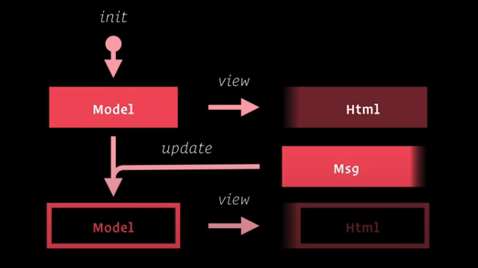
\includegraphics[width=0.75\textwidth]{elm-architecture}
\caption{Arquitectura Elm}
\end{figure}

Para realizar peticiones HTTP se amplía la arquitectura: tanto la función \code{init} como \code{update} pueden opcionalmente devolver un comando que defina la petición HTTP. Cuando el entorno de ejecución recibe la respuesta de la petición, genera un mensaje que es pasado como argumento a la función \code{update}.
\begin{figure}[h]
\centering
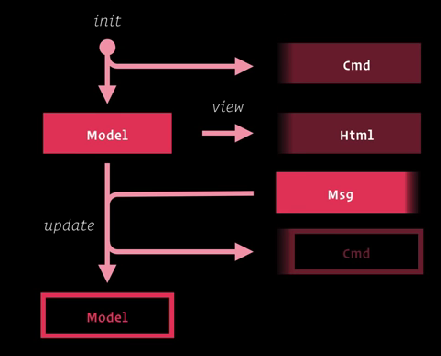
\includegraphics[width=0.7\textwidth]{complete-elm-architecture}
\caption{Arquitectura Elm completa}
\end{figure}

\pagebreak
\section{Corolario}
En la programación funcional, la lógica está estrictamente separada de los datos. No se tiene el concepto de ``datos que pueden hacer cosas" \medspace como en la programación orientada a objetos, sino que se tiene el concepto de ``funciones que manejan datos". El núcleo de la programación funcional es la composición, poder crear funciones complejas a partir de otras simples. Tener separados los datos de la lógica hace que la composición sea fácil: el resultado de combinar una función que calcula raíces cuadradas con la función \code{map} es una función que calcula las raíces cuadradas de cada elemento de un arreglo. La composición de un dato al que se le puede calcular su raíz cuadrada con un dato que puede aplicar una transformación a sus datos internos no es tan directa y tiene más \textit{boilerplate}.

Las funciones de orden superior hacen que la composición sea simple y expresiva, la inmutabilidad hace que sea segura y la transparencia referencial hace que sea predecible. En este documento faltó hablar de recursión para que se tengan las mismas características al hacer ciclos. 

La composición de datos también es un tema importante que no fue abarcado en este documento. Los sistemas de tipos de datos en lenguajes de programación funcional llegan a ser bastante simples y expresivos. Scott Wlaschin considera que esos tipos de datos son los ideales para hacer \textit{domain modeling}\cite{domain-modeling-fp}.

Es cierto que se puede programar con un estilo funcional sin saber sus raíces matemáticas, pero también es cierto que algo de conocimiento sobre teoría de categorías puede ayudar a entender la programación funcional a fondo.


\pagebreak
\begin{thebibliography}{99}
\bibitem{compilers-and-interpreters} \href{https://youtu.be/_C5AHaS1mOA}{Boiteau, D. (Escritor), y Beecroft, S. (Director). (1983). Computer Languages (Temporada 1, Episodio 6) [Episodio de programa de televisión]. En M. McManus (Productor ejecutivo), \textit{Bits and Bytes}. TVOntario.}

\bibitem{why-js} \href{https://medium.com/javascript-scene/why-learn-functional-programming-in-javascript-composing-software-ea13afc7a257}{Elliot, E. (20 de febrero de 2017). \textit{Why Learn Functional Programming in JavaScript?}. Medium. https://medium.com/javascript-scene/why-learn-functional-programming-in-javascript-composing-software-ea13afc7a257}

\bibitem{scope} \href{https://github.com/getify/You-Dont-Know-JS/blob/1st-ed/scope\%20\&\%20closures/README.md\#you-dont-know-js-scope--closures}{Simpson, K. (2014) \textit{You Don't Know JS: Scope \& Closures}. O'Reilly Media, Inc.}

\bibitem{functions} \href{https://developer.mozilla.org/es/docs/Web/JavaScript/Guide/Functions}{Developer.mozilla.org (15 de noviembre del 2021). \textit{Funciones - JavaScript | MDN}. https://developer.mozilla.org/es/docs/Web/JavaScript/Guide/Functions}

\bibitem{elixir-pattern-match} \href{https://elixir-lang.org/getting-started/pattern-matching.html}{The Elixir Team. (2012-2021). \textit{Pattern matching - The Elixir programming language}. https://elixir-lang.org/getting-started/pattern-matching.html}

\bibitem{elm-case} \href{https://elmprogramming.com/case-expression.html}{Poudel, P. (2018). \textit{Case Expression - Beginning Elm}. https://elmprogramming.com/case-expression.html}

\bibitem{why-isnt-fp-norm} \href{https://clojutre.org/2019/#feldman}{Feldman, R. (26-27 de septiembre de 2019). \textit{Why Isn't Functional Programming the Norm?} [Sesión de conferencia]. ClojuTRE, Helsinki, Finlandia. https://clojutre.org/2019/\#feldman}

\bibitem{mainstream-elm} \href{https://youtu.be/oYk8CKH7OhE}{Czaplicki, E. (6-7 de junio de 2015). \textit{Let's be mainstream! User focused design in Elm} [Discurso principal]. Curry On, Praga, República Checa. https://youtu.be/oYk8CKH7OhE}

\bibitem{skeptics-functional-style} \href{https://youtu.be/oF9XTJoScOE}{Mills, J. (21 de julio de 2017). \textit{A Skeptics Guide To Functional Style JavaScript} [Sesión de conferencia]. NEJS CONF, Omaha, Nebraska, Estados Unidos de América. https://youtu.be/oF9XTJoScOE}

\bibitem{fp-toolkit} \href{https://youtu.be/Nrp_LZ-XGsY}{Wlaschin, S. (28 de enero-1 de febrero de 2019). \textit{The Functional Programmer's Toolkit} [Sesión de conferencia]. NDC Conferences, Londres, Inglaterra. https://youtu.be/oF9XTJoScOE}

\bibitem{immutable-data-structures} \aparef{https://youtu.be/Wo0qiGPSV-s}{Vakil, A. (6-7 de mayo de 2017). \textit{Immutable data structures for functional JS} [Sesión de conferencia]. JSConf EU, Berlín, Alemania.}

\bibitem{dont-be-scared-of-fp} \aparef{https://youtu.be/XrNdvWqxBvA}{Hughes, J. (13-16 de octubre de 2016). \textit{Why Functional Programming Matters} [Discurso principal]. Functional Conf, Bangalore, Karnataka, India.}

\bibitem{memoize} \aparef{https://github.com/getify/Functional-Light-JS/blob/master/manuscript/ch5.md/}{Simpson, K. (Mayo 2019). \textit{Functional-Light JavaScript}. Manning.}

\bibitem{persistent-data-structures} \aparef{https://www.infoq.com/presentations/Value-Identity-State-Rich-Hickey/}{Hickey, R. (1 de octubre de 2009). \textit{Persistent Data Structures and Managed References} [Sesión de conferencia]. QCon, Londres, Inglaterra.}

\bibitem{functional-architecture} \aparef{https://youtu.be/US8QG9I1XW0}{Seemann, M. (2016). \textit{Functional architecture – The pits of success} [Sesión de conferencia]. NDC Conferences, Sídney, Australia.}

\bibitem{developer-happiness-elm} \aparef{https://youtu.be/kuOCx0QeQ5c}{Yank, K. (25 de mayo de 2017). \textit{Developer Happiness on the Front End with Elm} [Vídeo].}

\bibitem{redux-elm} \aparef{https://redux.js.org/understanding/history-and-design/prior-art\#elm}{The Redux documentation authors. (25 de junio de 2021). \textit{Prior Art}. Recuperado el 25 de noviembre de 2021}

\bibitem{vuex-elm} \aparef{https://v3.vuejs.org/guide/state-management.html}{v3.vuejs.org. (26 de mayo de 2021). \textit{State Management}. Recuperado el 25 de noviembre de 2021}

\bibitem{domain-modeling-fp} \aparef{https://youtu.be/1pSH8kElmM4}{Wlaschin, S. (14-18 de agosto de 2017). \textit{Domain Modeling Made Functional} [Sesión de conferencia]. NDC Conferences, Sídney, Australia.}

\end{thebibliography}

\end{document}